\section{Experimentación}

Dada la cantidad de vértices, los grafos se generan en el formato estándar DIMACS \footnote{Para ver algunos ejemplos del formato: http://mat.gsia.cmu.edu/COLOR/instances.html}. El generador toma como parámetro la densidad del grafo. Dada una clique con esa cantidad de vértices, se elijen vértices al azar hasta que se llega a la densidad deseada. Debido a que estas instancias están diseñadas para coloreo de grafos, asignamos los vértices de forma uniforme en el total de particiones pasado por parámetro a nuestro programa de coloreo particionado.

Por cuestiones de tiempo, cada uno de los experimientos CPLEX fue ejecutado sin límite de cantidad de threads, con un procesador Intel(R) Core(TM) i7-3610QM CPU @ 2.30GHz y 16GB de memoria RAM.

\subsection{Eliminación de simetría}

Al igual que el problema de coloreo de grafos, el problema del coloreo particionado de grafos presenta una gran cantidad de soluciones simétricas. De no romper la simetría del problema, los algoritmos tendrían un espacio de búsqueda mucho mayor, moviéndose por soluciones que, siendo computacionalmente distintas, en la práctica se trata de la misma. Esto afecta el tiempo de ejecución de forma considerable a medida que crece el tamaño del problema. Para romper la simetría en nuestro problema, en la sección \ref{simetria} mostramos cómo utilizamos la clásica condicion de coloreo de que los colores se deben utilizar en orden. Este fenómeno se puede ver en el siguiente gráfico:

\begin{figure}[h]
\centering
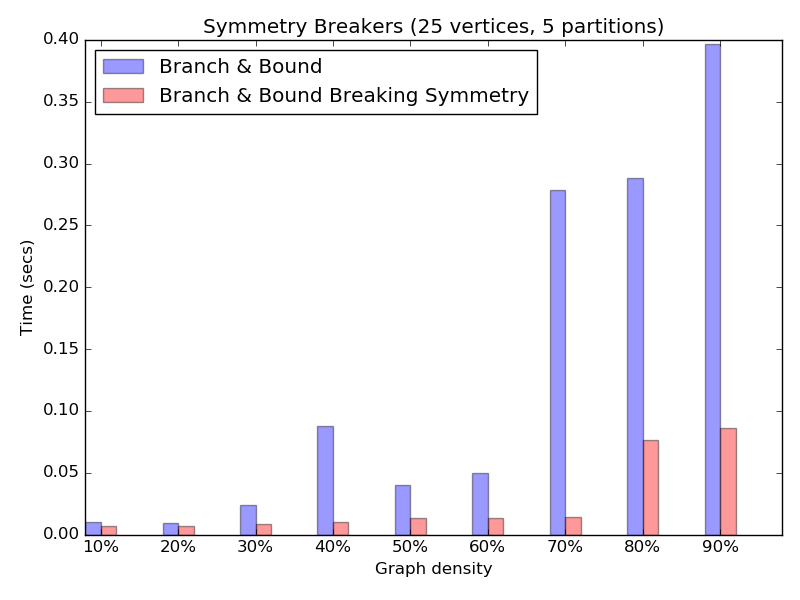
\includegraphics[scale=0.7]{img/2-symmetry_v25_p5_l40_t1_b0.png}
\caption{Tiempo de resolución del modelo incluyendo o no eliminación de simetría.}
\end{figure}

Esto nos brinda la noción sumamente relevante de la importancia y efectividad de romper simetría al realizar la formulación de un LP. Cabe mencionar que existen muchas otras estrategias o expresiones para disminuir aun más el grado de simetría de la formulación. La escogida bajo ninguna circunstancia debe ser considerada la mejor posible.

\pagebreak

\subsection{Efectividad de las familias de desigualdades}

La idea de este experimento es comparar las diferentes estrategias de planos de corte. Para ello, se eligió a 40 como la cantidad de cortes de cada tipo que se podían agregar, con una sola iteración:
% en cada iteración se podían agregar hasta 40 cortes?

\begin{figure}[h]
  \centering
  \begin{minipage}[b]{0.49\textwidth}
    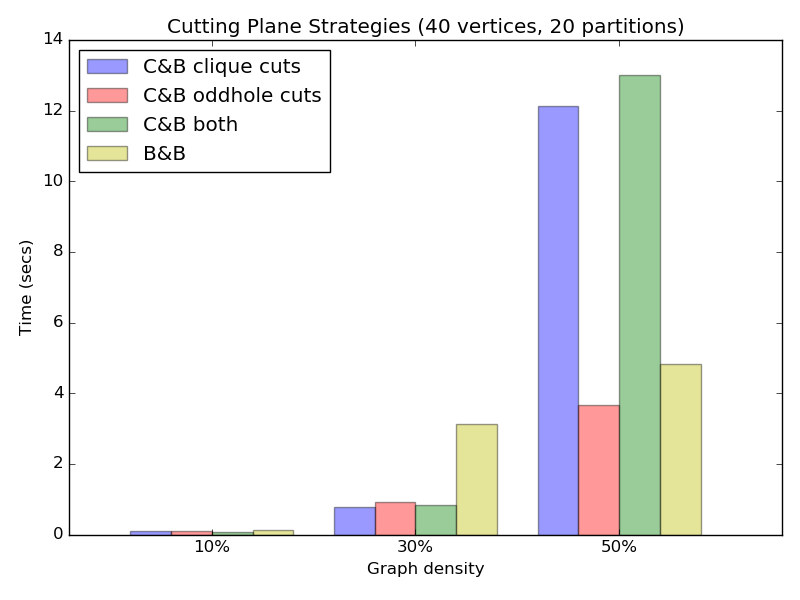
\includegraphics[width=\textwidth]{img/5-cuts_v40_p20_i1_l40_t1_b0.png}
    \caption{Estrategias de planos de corte (tiempo)}
  \end{minipage}
  \hfill
  \begin{minipage}[b]{0.49\textwidth}
    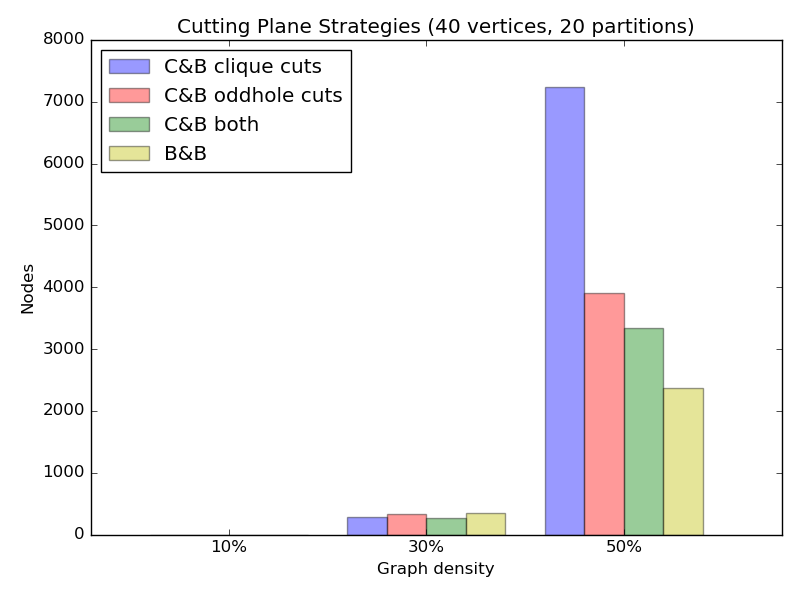
\includegraphics[width=\textwidth]{img/5-cuts_v40_p20_i1_l40_t1_b0_nodes.png}
    \caption{Estrategias de planos de corte (nodos recorridos)}
  \end{minipage}
\end{figure}

Lo primero que podemos observar es que no siempre hay una estrategia ganadora por sobre las otras. Se observa con claridad una dependencia entre la densidad del grafo y la estrategia que tuvo mejores resultados. Cuanto más denso, más cliques nuestra heurística debería encontrar, y a priori uno esperaría que los tiempos mejoren. Esto no sucede, de hecho agregar las restriciones de clique empeora el tiempo de ejecución con respecto al resultado de utilizar B\&B. También podemos observar que un mejor tiempo de ejecución no necesariamente implica que se recorren menos nodos en árbol de enumeración. En contra de lo que esperábamos inicialmente, las desigualdades de agujero impar parecen funcionar bien, aunque por supuesto esto se podría constatar con mayor peso de llevar a cabo una experimentación mas exhaustiva.

\subsection{Efecto de aumentar el número de particiones}

A medida que aumentamos el número de particiones, el problema comienza a parecerse más a uno de coloreo. Dado que las desigualdades que implementamos son clásicas de coloreo, es de esperar que la performance mejore a medida que aumenta el número de particiones \cite{coloring}. Para Cut \& Branch, sólo utilizamos los mejores 40 cortes de clique con una iteración. A medida que aumenta el número de particiones, podemos observar cómo la ganancia del corte es mayor.

\begin{figure}[h]
  \centering
  \begin{minipage}[b]{0.49\textwidth}
    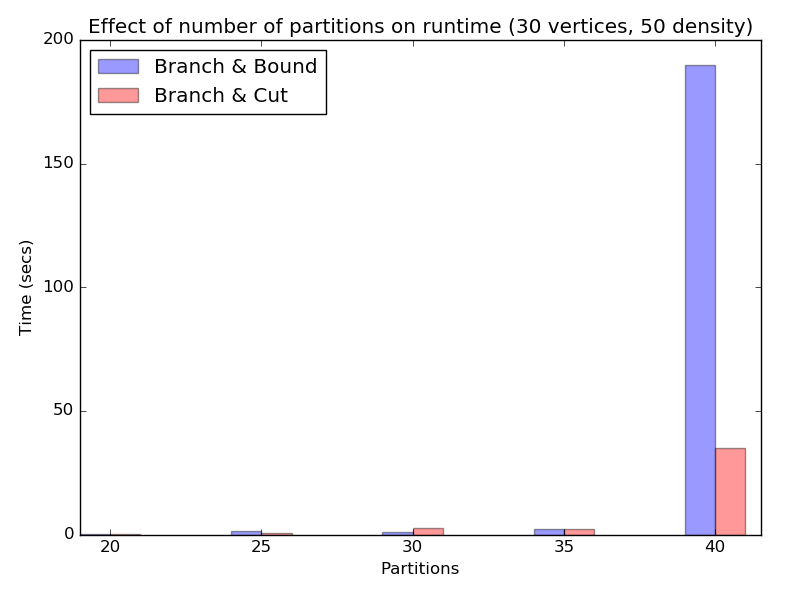
\includegraphics[width=\textwidth]{img/3-partitions_v30_d50_i1_co0_l40_t1_b0.png}
    \caption{Tiempo de ejecucion a medida que aumenta el numero de particiones.}
  \end{minipage}
  \hfill
  \begin{minipage}[b]{0.49\textwidth}
    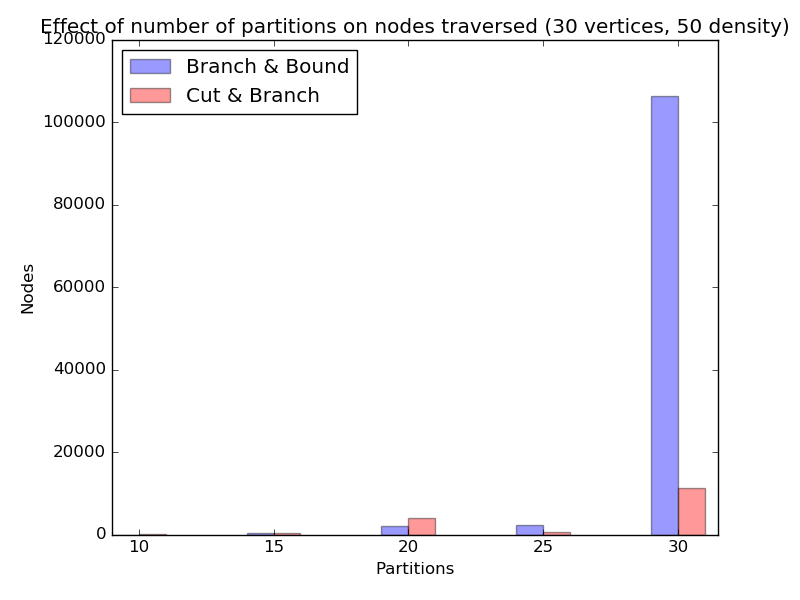
\includegraphics[width=\textwidth]{img/3-partitions_v30_d50_i1_co0_l40_t1_b0_nodes.png}
    \caption{Nodos recorridos a medida que aumenta el numero de particiones.}
  \end{minipage}
\end{figure}

\pagebreak

\subsection{Efecto de aumentar la densidad del grafo}

\begin{figure}[h]
  \centering
  \begin{minipage}[b]{0.49\textwidth}
    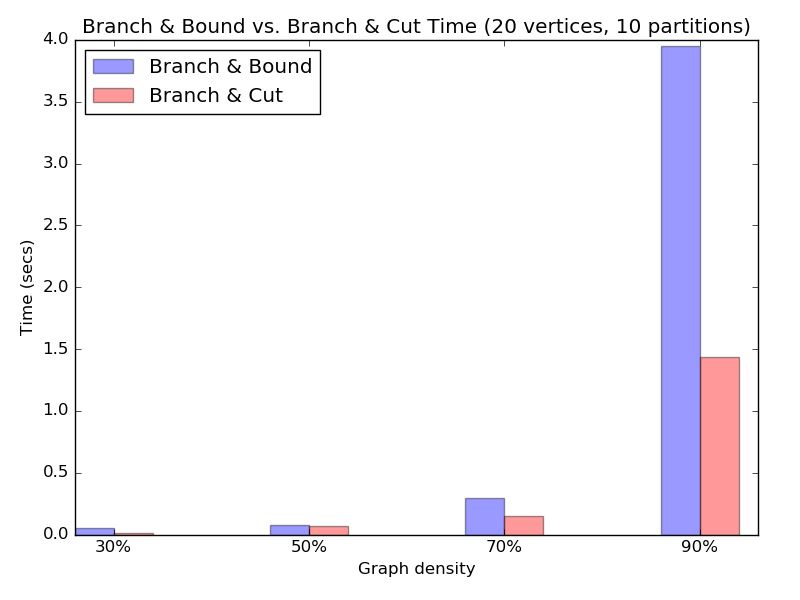
\includegraphics[width=\textwidth]{img/1-bb_vs_bc_v20_p10_i1_co0_l40_t1_b0.png}
  \end{minipage}
  \hfill
  \begin{minipage}[b]{0.49\textwidth}
    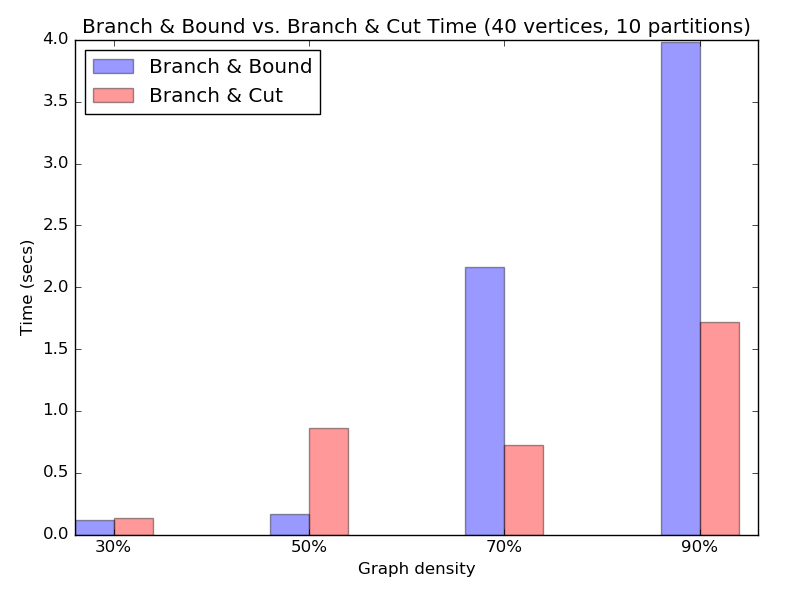
\includegraphics[width=\textwidth]{img/1-bb_vs_bc_v40_p10_i1_co0_l40_t1_b0.png}
  \end{minipage}
  \begin{minipage}[b]{0.49\textwidth}
    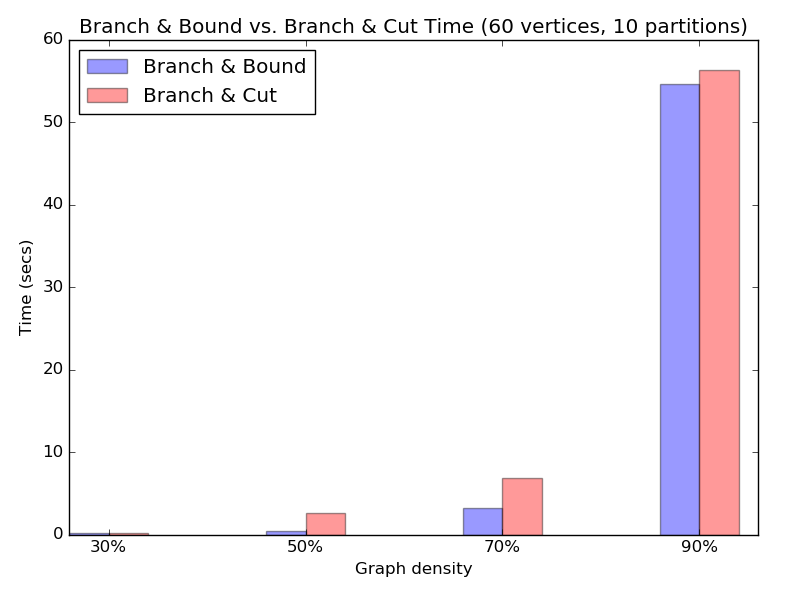
\includegraphics[width=\textwidth]{img/1-bb_vs_bc_v60_p10_i1_co0_l40_t1_b0.png}
  \end{minipage}
  \hfill
  \begin{minipage}[b]{0.49\textwidth}
    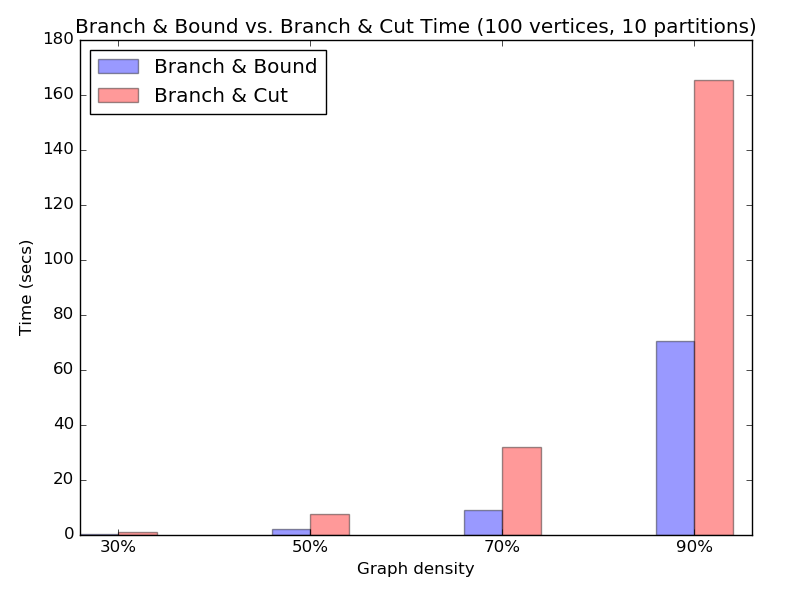
\includegraphics[width=\textwidth]{img/1-bb_vs_bc_v100_p10_i1_co0_l40_t1_b0.png}
  \end{minipage}
	\caption{Efecto de aumentar la densidad del grafo.}
\end{figure}

A medida que aumenta la densidad del grafo, el problema de coloreo se vuelve sin duda más difícil. En los casos donde el número de particiones es mayor en relación al numero de vértices, Branch \& Cut con 1 iteración y 40 desigualdades violadas parece funcionar mejor. Esto no sucede en grafos esparsos, donde Branch \& Bound puro tiene un menor tiempo de ejecución.

\pagebreak

\subsection{Efecto de aumentar la cantidad de restricciones incorporadas por iteración}

Para todos nuestros experimentos en general utilizamos sólo 1 iteración con un límite de 40 desigualdades por familia. La idea de este experimento es evaluar esta configuración. Para ello, utilizamos un grafo con 40 vértices y 20 particiones.

\begin{figure}[h]
  \centering
  \begin{minipage}[b]{0.49\textwidth}
    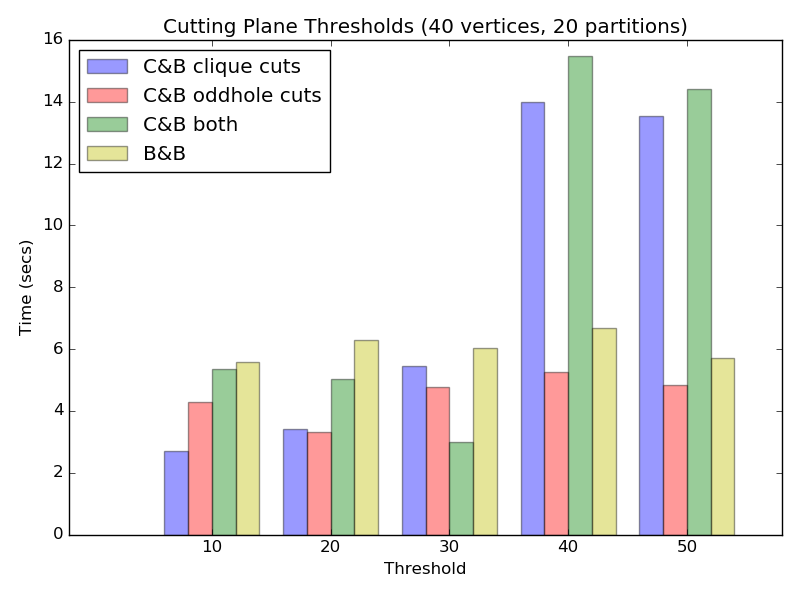
\includegraphics[width=\textwidth]{img/6-thresholds_v40_p20_i1_t1_b0.png}
    \caption{Tiempo de ejecución al incrementar el número de restricciones incorporadas.}
  \end{minipage}
  \hfill
  \begin{minipage}[b]{0.49\textwidth}
    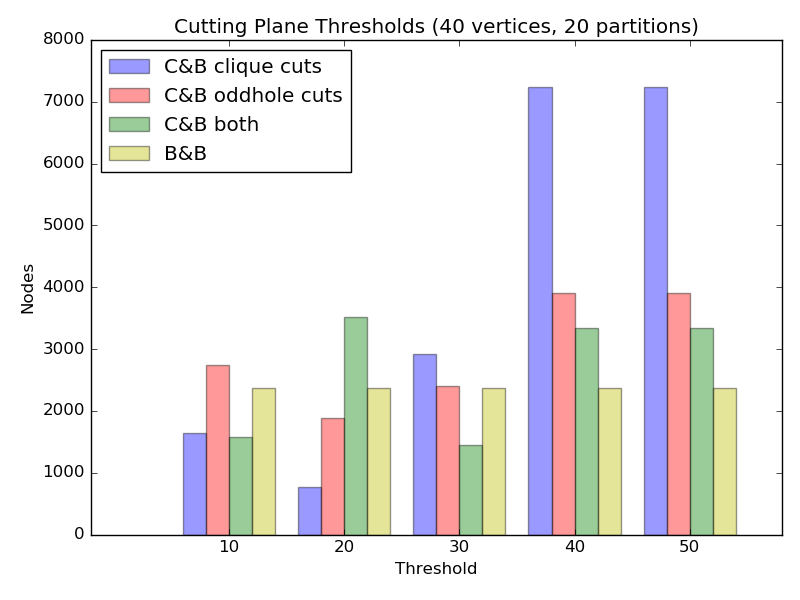
\includegraphics[width=\textwidth]{img/6-thresholds_v40_p20_i1_co2_t1_b0_nodes.png}
    \caption{Nodos recorridos al incrementar el número de restricciones incorporadas.}
  \end{minipage}
\end{figure}

Como podemos observar, agregar más restricciones no es siempre ventajoso. En un principio, agregar restricciones parece mejorar la ejecución del C\&B, pero ya a partir de 40 el tiempo de ejecución empeora de forma abrupta para las cliques. Esto no sucede para las restricciones de agujero impar. Nuevamente, esto se puede deber a que nuestra heurística de clique no es lo suficientemente buena.

\subsection{Efecto de aumentar la cantidad de iteraciones de planos de corte}

\begin{figure}[h]
\centering
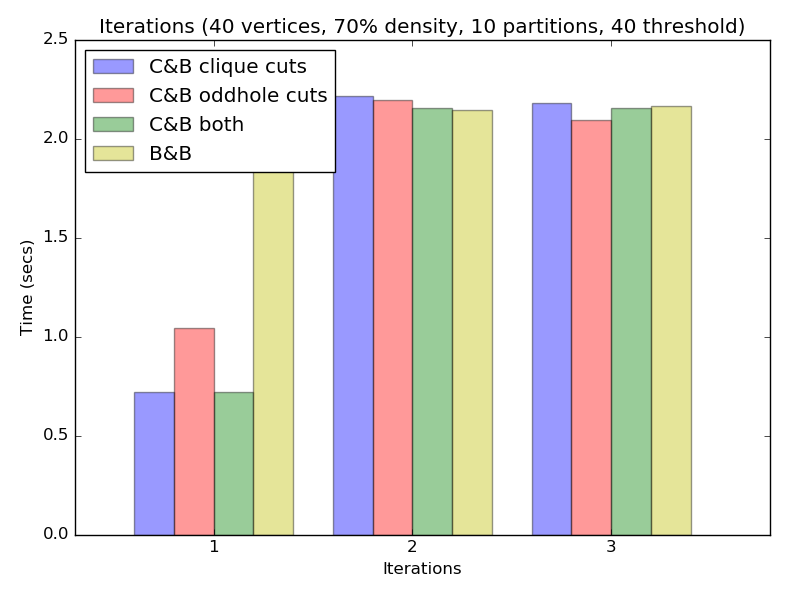
\includegraphics[scale=0.5]{img/7-iterations_v40_p10_l40_t1_b0.png}
\caption{Tiempo de ejecución al aumentar la cantidad de iteraciones de planos de corte.}
\end{figure}

Como podemos ver, aumentar el numero de iteraciones de planos de corte no necesariamente mejora el tiempo de ejecución. En cada iteración lo que hacíamos era generar una familia en función de la solución de la relajación del problema, y luego agregar las \textit{mejores} restricciones. En relación a la sección anterior, esto también esta relacionado con el $threshold$ que elegimos para hacer la experimentación.

\pagebreak

\subsection{Comparación B\&B, C\&B, CPLEX default}

\begin{figure}[h]
  \centering
  \begin{minipage}[b]{0.49\textwidth}
    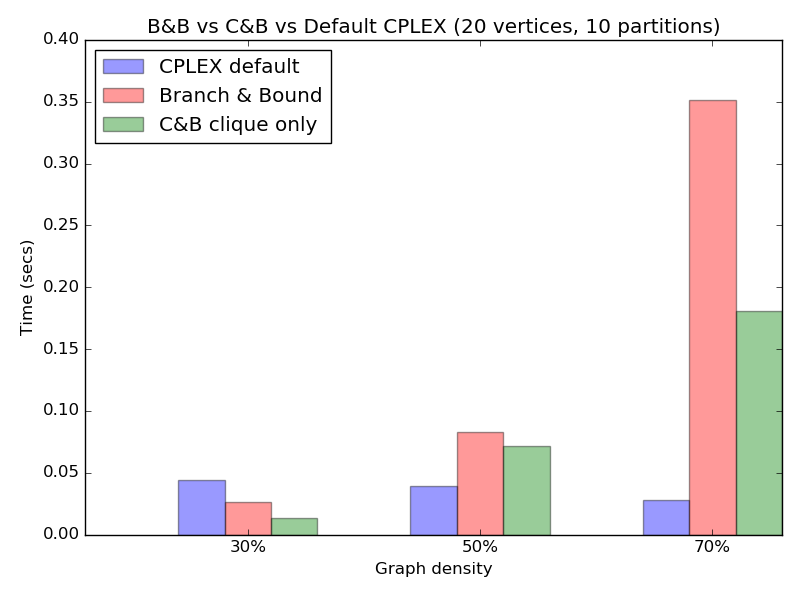
\includegraphics[width=\textwidth]{img/8-compare_v20_p10_i1_l40_t1_b0.png}
  \end{minipage}
  \hfill
  \begin{minipage}[b]{0.49\textwidth}
    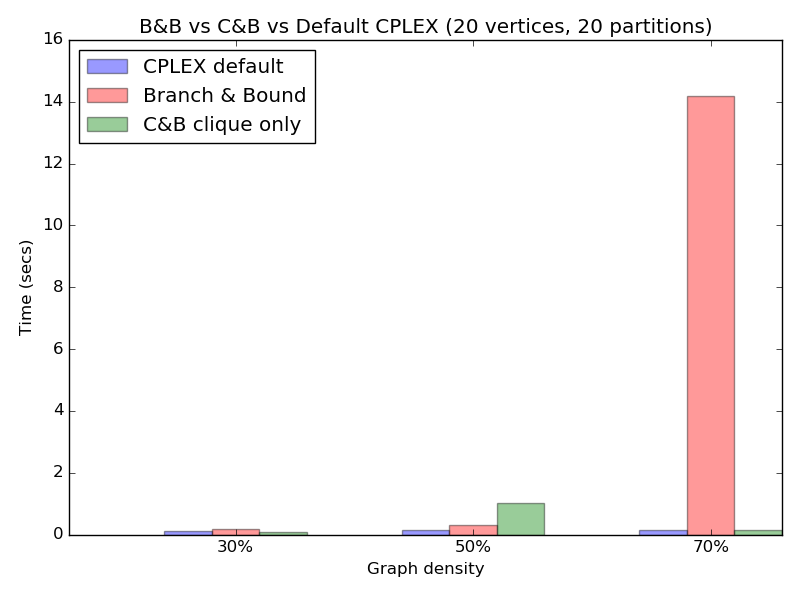
\includegraphics[width=\textwidth]{img/8-compare_v20_p20_i1_l40_t1_b0.png}
  \end{minipage}
  \begin{minipage}[b]{0.49\textwidth}
    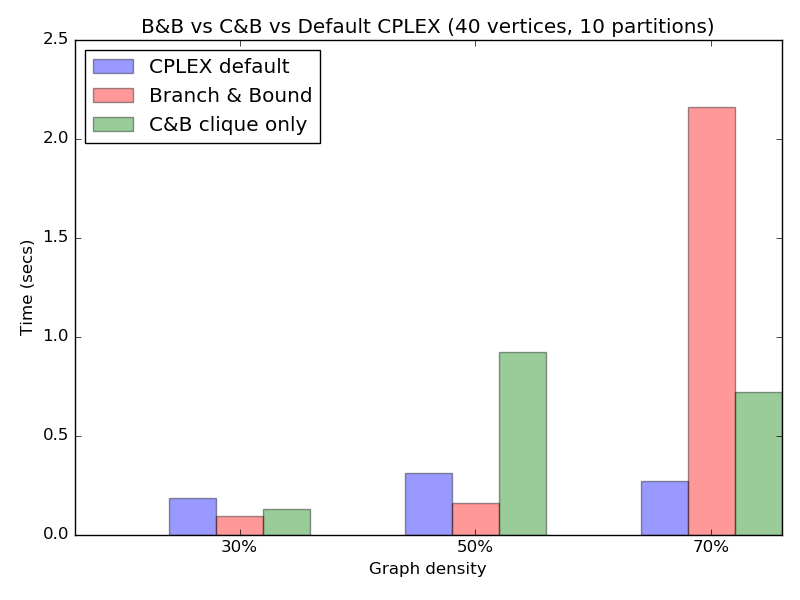
\includegraphics[width=\textwidth]{img/8-compare_v40_p10_i1_l40_t1_b0.png}
  \end{minipage}
  \hfill
  \begin{minipage}[b]{0.49\textwidth}
    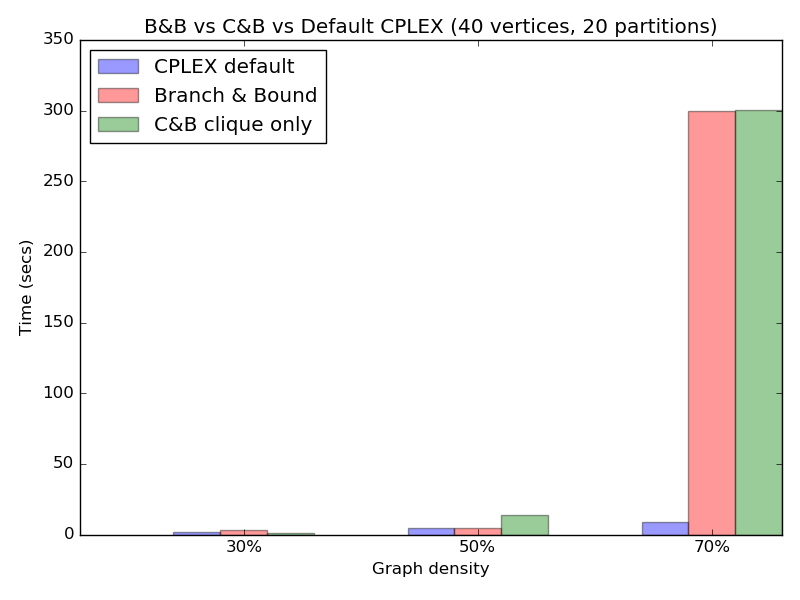
\includegraphics[width=\textwidth]{img/8-compare_v40_p20_i1_l40_t1_b0.png}
  \end{minipage}
	\caption{Comparacion B\&B, C\&B, CPLEX default para diferentes grafos.}
\end{figure}

Dado que el CPLEX por default utiliza cortes de Gomory y preprocesamiento de variables, no nos sorprende que en general sea superior a nuestras otras estrategias para grafos densos. Una propuesta interesante podría ser repetir esta experimentación permitiendo los cortes y el preprocesamiento para todas nuestras estrategias. Otra observación, el gráfico superior derecho es el caso de coloreo de grafos, dado que cada vértice pertenece a una partición diferente. Aquí podemos ver que las desigualdades de clique son sumamente útiles. 

\pagebreak

\subsection{Estrategias de recorrido del árbol de enumeración
y selección de variable de branching}

Existen muchas estrategias de recorrido del árbol de enumeración. En este trabajo solo analizaremos DFS y BBS. DFS (Depth First Search) recorre el árbol de enumeración de B\&B primero en profundidad. Por otro lado, BBS (Best Bound Search) recorre el árbol de enumeración utilizando alguna estrategia para intentar buscar una buena cota lo mas rápido posible. En general se utilizan estrategias heurísticas. En el caso de CPLEX, dado un nodo padre se calcula la solución a la relajación de todos sus hijos y luego se continua recorriendo el nodo con el mayor resultado de la función objetivo. \footnote{http://www-01.ibm.com/support/knowledgecenter/SSSA5P\_12.6.1/ilog.odms.cplex.help/CPLEX/Parameters/topics/NodeSel.html}.

Ambas estrategias son sumamente ventajosas ya que permiten obtener una cota superior a la solución final para utilizar de poda al hacer backtracking sobre el árbol de enumeración. Dado que no utilizamos heurísticas iniciales, esta estrategia parece razonable. 

Por otro lado, las estrategias de selección de variable buscan encontrar cual es la mejor variable sobre la cual hacer branching. Hay muchas reglas, como por ejemplo \textit{max/min infeasibility}. Mientras que la regla de \textit{minimum infeasibility} busca hacer branching sobre mas cercana al entero, la regla de \textit{maximum infeasibility} busca hacer exactamente lo contrario \footnote{http://www-01.ibm.com/support/knowledgecenter/SS9UKU\_12.4.0/com.ibm.cplex.zos.help/Parameters/topics/VarSel.html}.

En esta sección analizaremos 4 combinaciones de estrategias de recorrido del árbol de enumeración y selección de variable de branching para B\&B puro y C\&B con cortes de clique, 1 iteración y $threshold = 30$. Las combinaciones que analizaremos son: DFS + MAXINFEAS, DFS + MININFEAS, BESTBOUND + MAXINFEAS, BESTBOUND + MININFEAS.

\begin{figure}[h]
  \centering
  \begin{minipage}[b]{0.49\textwidth}
    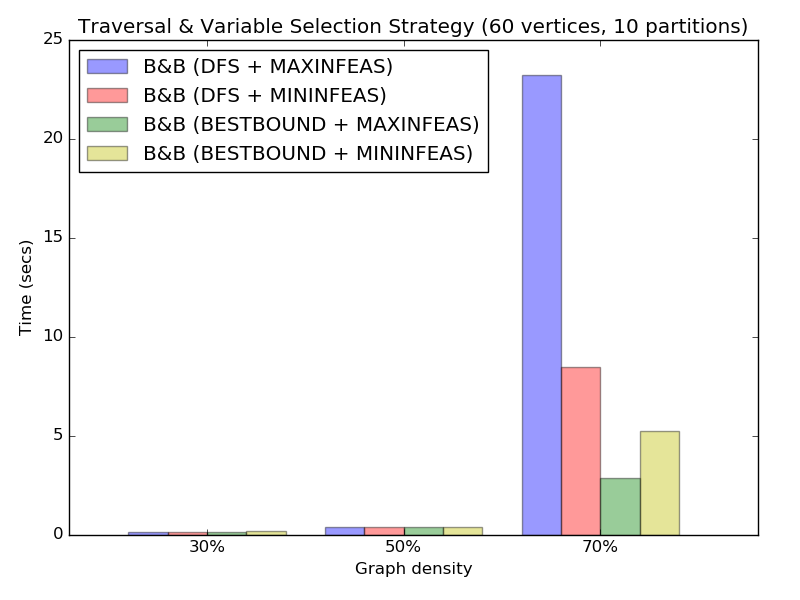
\includegraphics[width=\textwidth]{img/9-tree_v60_p10_i1_l30_s1.png}
  \end{minipage}
  \hfill
  \begin{minipage}[b]{0.49\textwidth}
    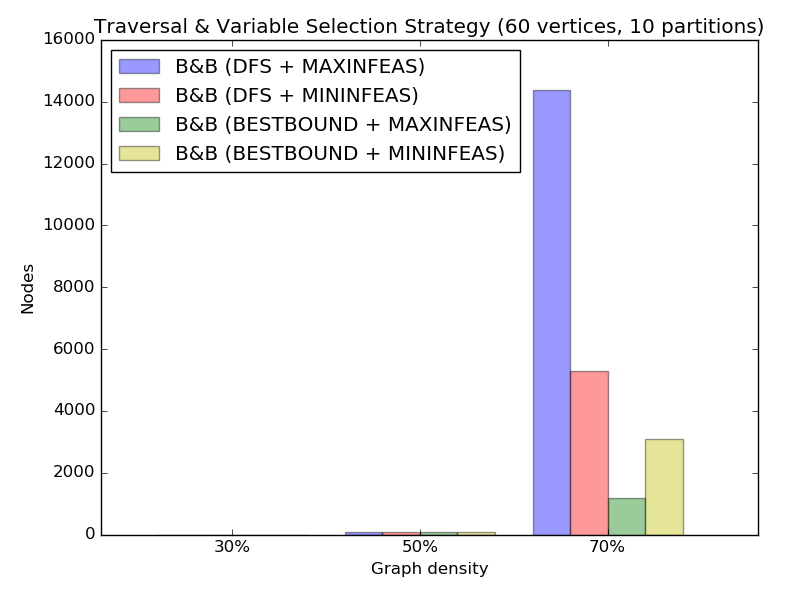
\includegraphics[width=\textwidth]{img/9-tree_v60_p10_i1_l30_s1_nodes.png}
  \end{minipage}
  \begin{minipage}[b]{0.49\textwidth}
    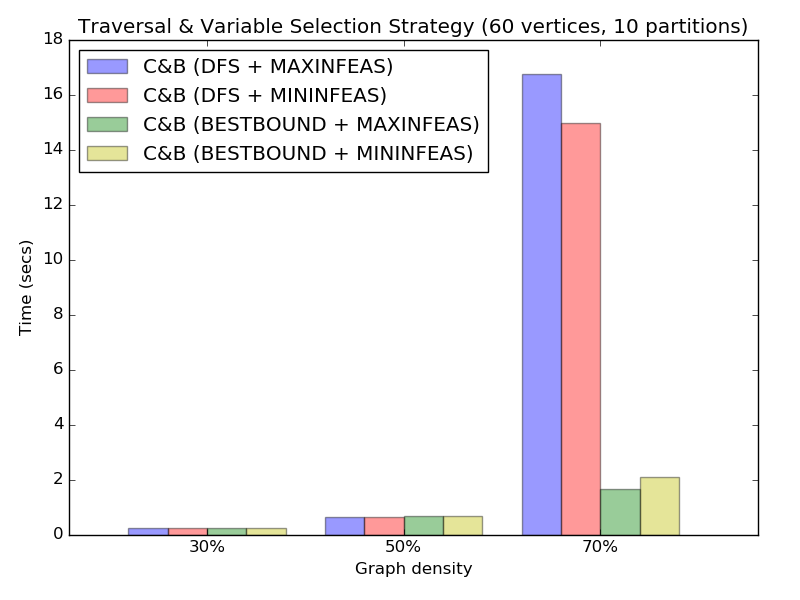
\includegraphics[width=\textwidth]{img/9-tree_v60_p10_i1_l30_s2.png}
  \caption{Tiempo de ejecución dependiendo de la estrategias de recorrido y selección de variable.}
  \end{minipage}
  \hfill
  \begin{minipage}[b]{0.49\textwidth}
    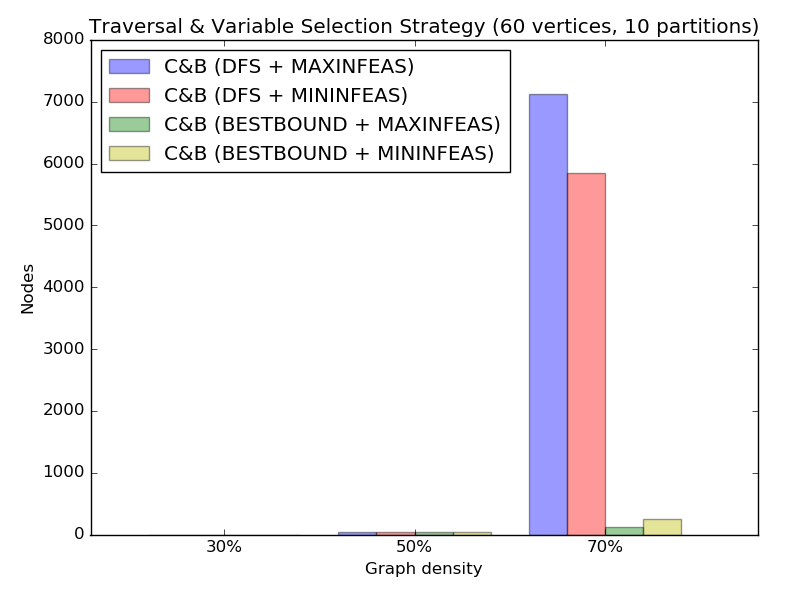
\includegraphics[width=\textwidth]{img/9-tree_v60_p10_i1_l30_s2_nodes.png}
  \caption{Nodos recorridos dependiendo de la estrategias de recorrido y selección de variable.}
  \end{minipage}
\end{figure}

Como podemos observar, en general C\&B tiene tiempos de ejecución menores y a su vez recorre menos nodos. La mejor estrategia para este problema parece ser BESTBOUND + MAXINFEAS. CPLEX utiliza por default BESTBOUND, aunque utiliza una heurística para elegir la variable de branching. 